%!TEX root = ../thesis.tex
%*******************************************************************************
%****************************** Third Chapter **********************************
%*******************************************************************************
\chapter{Reduced Order Modeling of Comb-Drive in Electrolytes}

% **************************** Define Graphics Path **************************
\ifpdf
    \graphicspath{{Chapter3/Figs/Raster/}{Chapter3/Figs/PDF/}{Chapter3/Figs/}}
\else
    \graphicspath{{Chapter3/Figs/Vector/}{Chapter3/Figs/}}
\fi

\section{Summary}
The focus of this chapter will be the development of reduced order models for the comb-drive actuator in electrolytes. We will first review the Poisson-Nernst-Planck equations for describing ionic liquids between parallel plates. This will be followed by a discussion of how these equations facilitate the conceptualization of the system as a circuit, and how this conceptualization was used to develop the classic model. In particular, the assumptions behind the classic model will be enumerated, as will it's shortcomings when fit to data. Finally, we will present our newly developed models, the assumptions behind this work, and opportunities for further work with regard to these models. 

\section{Poisson-Nernst-Planck (PNP) Equations}
We saw in Chapter 2 that modeling a comb-drive actuator in electrolytes reduces to modeling the overlapping regions of its fingers as parallel plates filled with a dilute ionic solution. This system is classically described by the Poisson-Nernst-Planck (PNP) equations. The one-dimensional PNP equations are

\begin{align}
    \frac{\partial c_\pm}{\partial t} = - D\frac{\partial}{\partial x}\bigg(-\frac{\partial c_\pm}{\partial x} \mp  \frac{ze}{k_B T}c_\pm \frac{\partial \phi}{\partial x}\bigg) \label{pnp_equations_1} \\
    -\epsilon \frac{\partial^2 \phi}{\partial x^2} = \rho_e = ze(c_+ - c_-) \label{pnp_equations_2} 
\end{align}
where $c_+$ and $c_-$ are the concentrations of the negative and positive ions respectively, $\phi$ is the electric potential, D is the diffusivity of the electrolyte, which is assumed to be constant throughout the domain, $z$ is the valence number of the electrolytes, $k_B$ is the Boltzmann constant, $T$ is the temperature of the domain, $\epsilon$ is the relative permittivity of the aqueous solution, $\rho_e$ is the electric charge density, and $e$ is the charge of an electron.

Before performing further analysis on the PNP equations, it is important that we do two things. First, we non-dimensionalize the PNP equations, and then we communicate the physical intuition of the resulting equations. We non-dimensionalize the PNP equations as was done by Druzgalski et al \cite{Druzgalski2013}. The potential, time, concentration, and spatial coordinates are non-dimensionalized as

\begin{equation}\label{nondim_quants}
    \phi^* = \frac{\phi}{V_T}, \quad t^* = \frac{Dt}{g^2}, \quad  c^*_0 = \frac{c}{c_0}, \quad  x^* = \frac{x}{g},
\end{equation}
where $V_T = \frac{k_B T}{e}$ is the thermal voltage, $g$ is the length of the gap between comb-drive fingers, $c_0$ is the bulk concentration of an ion, and the rest of the terms in the equation are defined after \ref{pnp_equations_1} and \ref{pnp_equations_2}. Using these terms, the non-dimensional form of the PNP equations is
\begin{align}
    \frac{\partial c_\pm^*}{\partial t^*} = - \frac{\partial}{\partial x^*}\bigg(-\frac{\partial c_\pm^*}{\partial x^*} \mp  c_\pm^* \frac{\partial \phi^*}{\partial x^*}\bigg) \label{pnp_equations_nondim_1} \\
    -2 \gamma^2 \frac{\partial^2 \phi^*}{\partial x^{*2}} = \rho_e^* = c_+^* - c_-^* \label{pnp_equations_nondim_2} 
\end{align}
where $\gamma = \frac{\lambda_d}{g}$. The summation in \ref{pnp_equations_nondim_1} is essentially the nondimensional current flux, $f_\pm^*$, of the positive and negative ions respectively.


\subsection{Circuit View of System using Linearized PNP Equations}
We have introduced and non-dimensionalized the PNP equations, as well as given physical intuition regarding its non-dimensional form. We will now use the non-dimensionalized PNP equations to explain the representation of electrolytes between parallel plates as a circuit. 

We first make the critical assumption that the voltage applied to the parallel plate is small. A small voltage is defined as a voltage that is at most the same order of magnitude as the thermal voltage, $V_T$, which is about 25 $\mV$. When the applied voltage is small, the region between the parallel plates is described as three distinct parts, figure \ref{conc_profile}. The center of the domain is called the bulk, and is characterized by an equal concentration of positive and negative ions, low concentration gradients, and a linear potential profile. The two regions located close to the parallel plates, however, are characterized by high concentration gradients, unequal amounts of positive and negative ions, and a nonlinear potential profile. The concentration of positive ions is much higher than the negative at the parallel plate with a lower potential, and vice versa at that with one that is higher. 

\begin{figure}[htpb]
    \begin{center}
    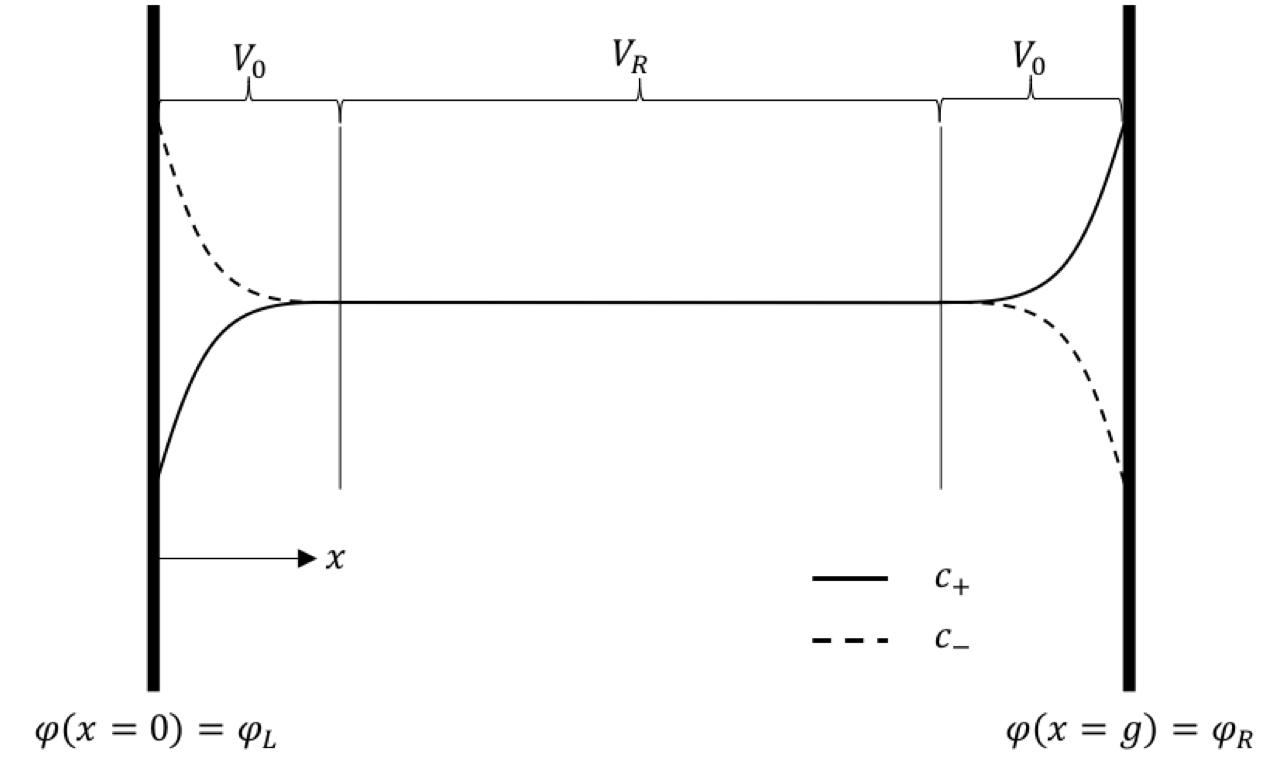
\includegraphics[width=0.7\linewidth]{Chapter3/figure/conc_profile.png}
    \caption{Schematic of concentration profile of negative and positive ions of electrolyte between parallel plates.}\label{conc_profile}
    \end{center}
\end{figure}

We can apply the non-dimensional PNP equations to these three regions separately, and use the assumption of a small applied voltage, to develop a circuit model for the system. We start with the bulk region in which the concentration gradient is zero, $\frac{\partial c_\pm^*}{\partial x^*} = 0$, and the potential profile is linear, $\frac{\partial \phi^*}{\partial x^*}=a \implies \frac{\partial^2 \phi^*}{\partial x^{*2}}=0$, where $a$ is some constant. Using these assumptions, \ref{pnp_equations_nondim_1} and \ref{pnp_equations_nondim_2} reduce to

\begin{align}
    \frac{\partial c_\pm^*}{\partial t^*} = - \frac{\partial}{\partial x^*}\bigg( \mp  c_\pm^* \frac{\partial \phi^*}{\partial x^*}\bigg) = 0 \label{pnp_equations_simple_nondim_1} \\
    -\gamma^2 \frac{\partial^2 \phi^*}{\partial x^{*2}} = \rho_e^* = c_+^* - c_-^* = 0\label{pnp_equations_simple_nondim_2} 
\end{align}

So, in the bulk we can assume that the concentration of positive and negative ions are equal, and that the concentration does not change as a function of time. We can now write the net current flux in the system as
\begin{align}
    j = f_+^* - f_-^* & = (c_+^* + c_-^*)\frac{\partial \phi^*}{\partial x^*} \label{bulk_current_flux_1} \\ 
    & = 2c_0^*\frac{\partial \phi^*}{\partial x^*} \label{bulk_current_flux_2}  
\end{align}
where \ref{bulk_current_flux_2} is obtained by using the fact that $c_+^* = c_-^*=c_0^*=1$ in the bulk. Equation \ref{bulk_current_flux_2} has the form $I=\frac{V}{R}$. We can, therefore, view the non-dimensional resistance and voltage of the bulk region, respectively, as 

\begin{equation} \label{bulk_resist_volt}
    R_{Bulk}^* = \frac{1}{2c_0^*}, \quad V_{Bulk}^* = \int_{0}^{g} \frac{\partial \phi^*}{\partial x^*} dx^*.
\end{equation}

We can perform a similar analysis on the electric double layer regions between the parallel plates. In this region, the poisson equation is 
\begin{align}
    -\gamma^2 \frac{\partial^2 \phi^*}{\partial x^{*2}} & = c_+^* - c_-^* = \rho_e^* \label{poisson_nondim_cap_1} \\
    &  = \text{sinh}(\frac{\phi^*}{2}) = \frac{dq^*}{dx^*}\nonumber
\end{align}
where \ref{poisson_nondim_cap_1} is obtained by assuming a boltzmann distribution.
\begin{equation} \label{boltzmann_distrib}
    c_+^* = c_0^* e^{-\frac{\phi z e}{k_B T}}, \quad c_-^* = c_0^* e^{\frac{\phi z e}{k_B T}}
\end{equation}
 Under the assumption of linearity, we rewrite \ref{poisson_nondim_cap_1} as  
\begin{equation}\label{poisson_nondim_ode}
\gamma^2 \frac{d^2\phi^*}{dx^{*2}} - \phi^* =0.
\end{equation}.
Solving this ODE, and taking a first order derivative of it's solution, yields
\begin{equation} \label{poisson_nondim_odesol}
\frac{d\phi^*}{dx^*} = -\gamma^{-1} \phi^*,
\end{equation}
We now rewrite \ref{poisson_nondim_cap_1}, using the solution of \ref{poisson_nondim_ode}, as
\begin{equation} \label{poisson_nondim_odesol_charge}
-2 \bigg(\frac{\lambda_d}{g}\bigg)^2 \frac{d^2\phi^*}{dx^{*2}} = -2 \phi^* = \frac{dq^*}{dx^*}
\end{equation}
Equations \ref{poisson_nondim_odesol} and \ref{poisson_nondim_odesol_charge} indicate that the boundary regions between the electrolytes can be represented as a capacitor. We obtain the dimensionless linear differential capacitance of this region by taking the quotient of \ref{poisson_nondim_odesol} and \ref{poisson_nondim_odesol_charge}, yielding
\begin{equation} \label{lin_diff_cap}
\frac{dq^*}{dx^*}\frac{dx^*}{d\phi^*} = \frac{dq^*}{d\phi^*} = 2\frac{\lambda_d}{g} = 2\gamma = C_0 
\end{equation}

Based on this analysis, it is clear that we can view electrolytes between parallel plates as a circuit composed of boundary oxide capacitors, and a bulk resistor, figure \ref{classic_circuit}.

\section{Classic Circuit Model of Comb-Drive Actuator in Electrolyte}
In this section, we will discuss the classic model of the comb-drive in electrolytes, which is based on the circuit model derived in the previous section, figure \ref{classic_circuit}.

\begin{figure}[htpb]
    \centering
    \begin{minipage}{\textwidth}
        \centering
        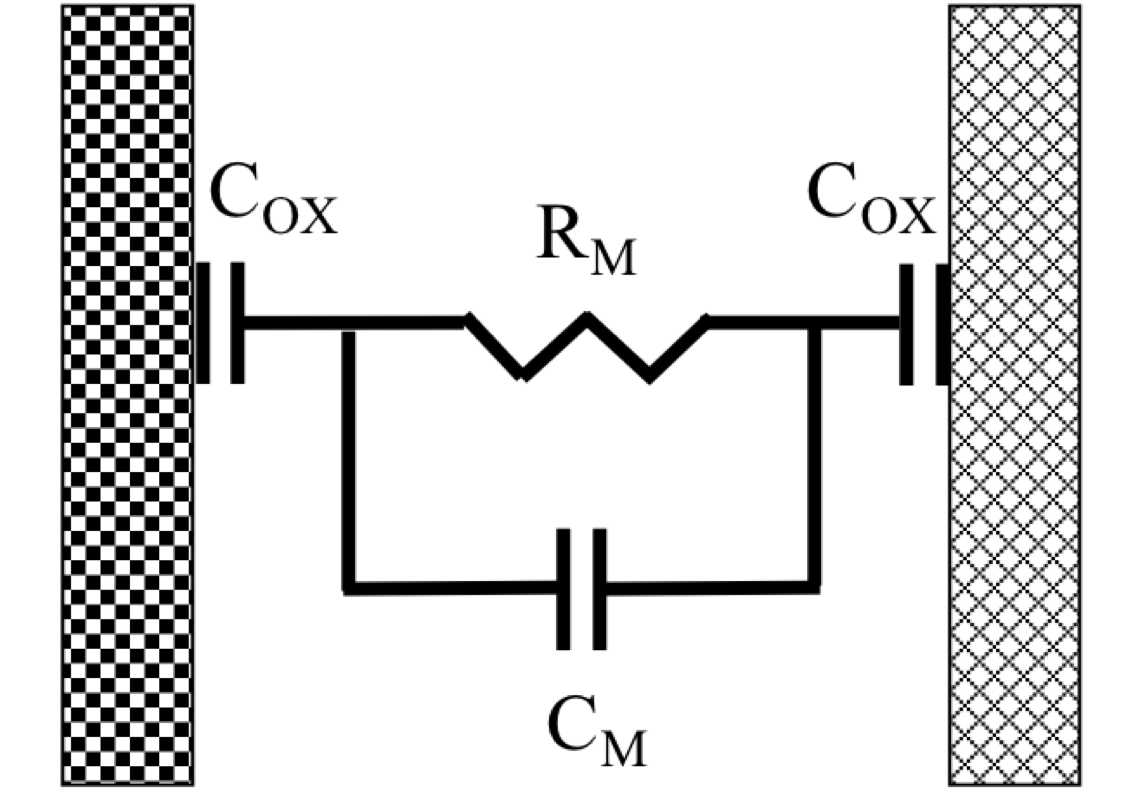
\includegraphics[width=0.6\textwidth]{Chapter3/figure/classic_circuit.png} % first figure itself
        \caption{Circuit schematic of the classic circuit model for describing a comb-drive actuator in electrolytes. It is composed of an oxide capacitor at the boundary, and a parallel resistor/capacitor in the bulk.}\label{classic_circuit}
    \end{minipage}\vfill
    \begin{minipage}{\textwidth}
        \centering
        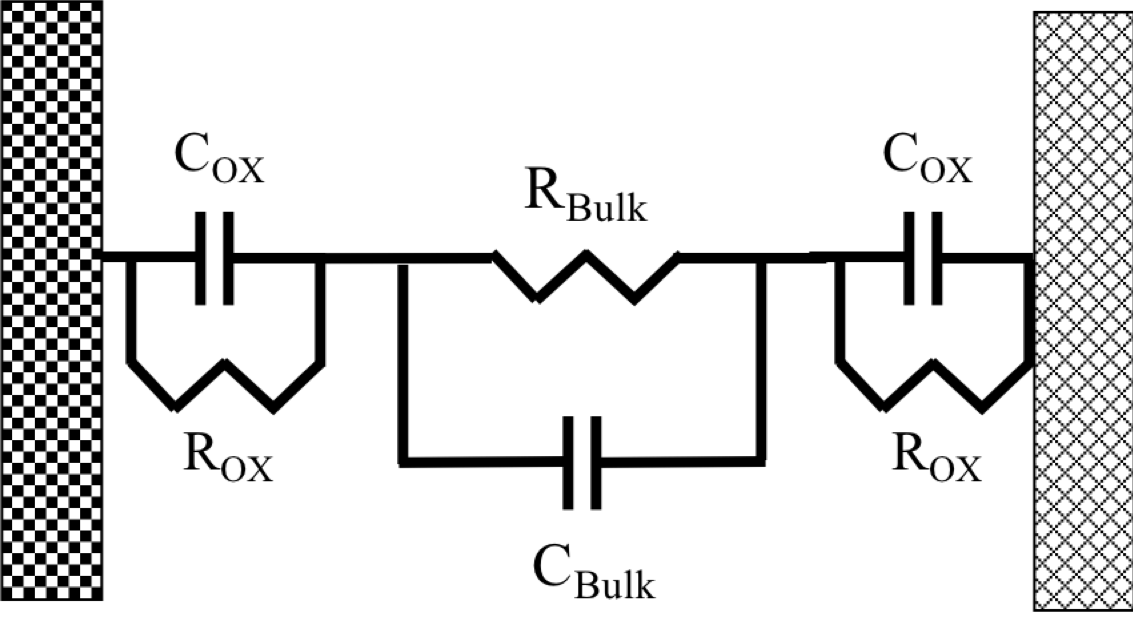
\includegraphics[width=0.8\textwidth]{Chapter3/figure/leaky_ox_circuit.png} % second figure itself
        \caption{Circuit schematic of the leaky circuit model for describing a comb-drive actuator in electrolytes. In this case the boundary is composed of a parallel resistor and capacitor to represent the oxide.}\label{leaky_ox_circuit}
    \end{minipage} \vfill
    \begin{minipage}{\textwidth}
        \centering
        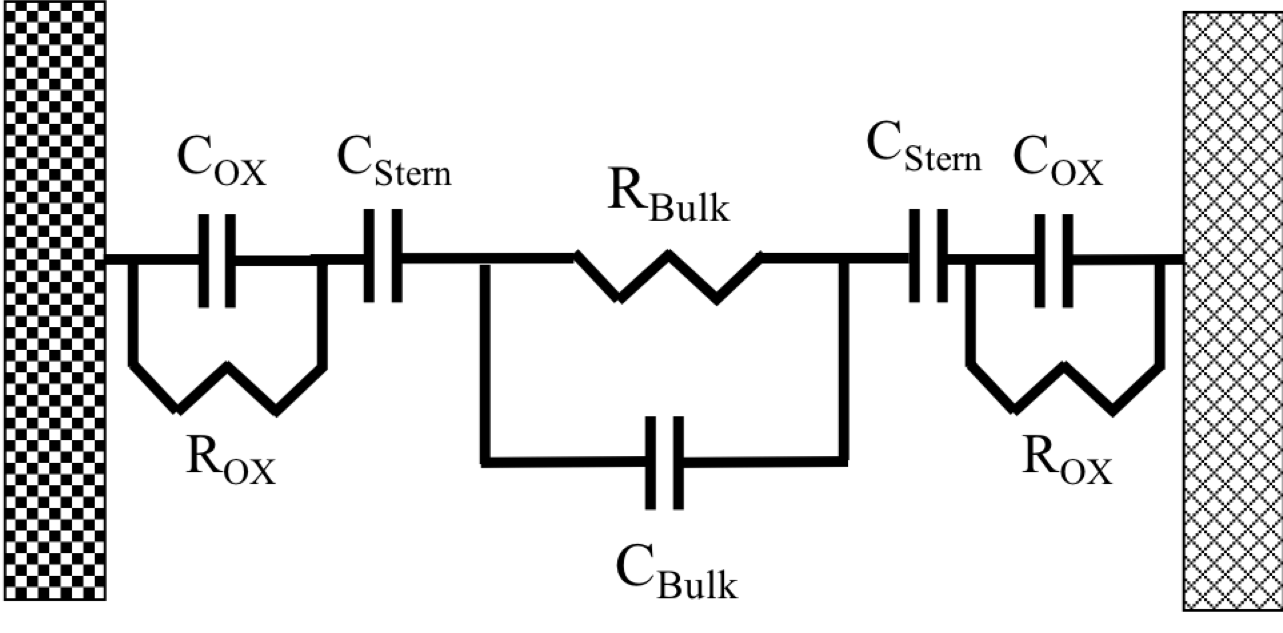
\includegraphics[width=0.8\textwidth]{Chapter3/figure/leaky_ox_stern_circuit.png} % second figure itself
        \caption{Circuit schematic of the leaky circuit model for describing a comb-drive actuator in electrolytes. It is similar to the leaky oxide schematic, except a stern layer is placed in series with the oxide resistor/capacitor.}\label{leaky_ox_stern_circuit}
    \end{minipage} \vfill
\end{figure}

\begin{comment}
\begin{figure}[htpb]
    \begin{center}
    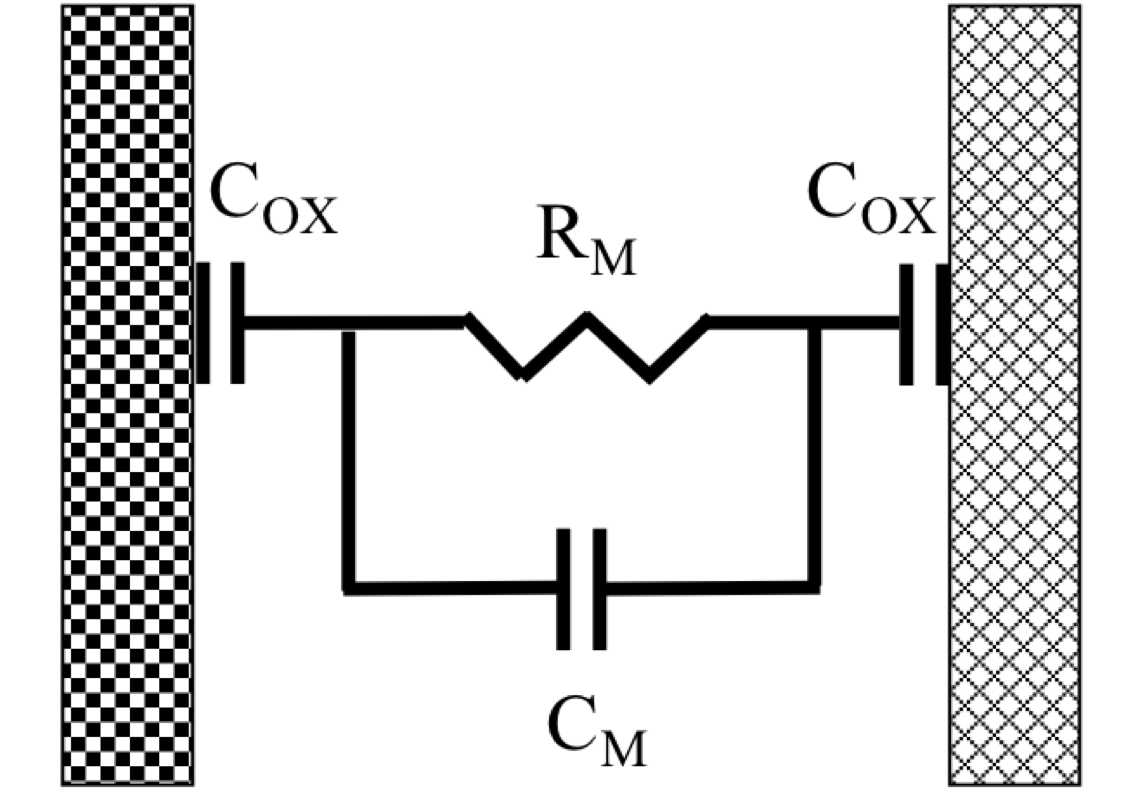
\includegraphics[width=0.7\linewidth]{Chapter3/figure/classic_circuit.png}
    \caption{Circuit schematic of the classic circuit model for describing a comb-drive actuator in electrolytes. It is composed of an oxide capacitor at the boundary, and a parallel resistor/capacitor in the bulk.}\label{classic_circuit}
    \end{center}
\end{figure}
\end{comment}

The force, $F$, experienced by a comb-drive actuator in air can be calculated as
\begin{equation}\label{air_force_comb} 
F = kx = \dfrac{Nb\epsilon_0}{g}V_{App}^2,
\end{equation}
where \textit{k}, the stiffness of the comb-drive, \textit{x}, its displacement, \textit{N}, the total number of comb-pair fingers, \textit{b}, the comb finger thickness (into the page), and \textit{g}, the distance between overlapping fingers, are properties of the comb-drive.  $\epsilon_0$ is the permittivity of free space, and $V_{App}$ is the voltage applied to an overlapping pair of fingers. In this scenario, fringe effects of the comb-drive tip can be ignored. This simplified model is most accurate with sufficient overlap between fingers\cite{Ye1998}. The classic model constructed by Mukundan et al. and Panchawagh et al. can be expressed by modifying \ref{air_force_comb} \cite{MukundanandPonce2009,Panchawagh2009},
\begin{equation}\label{classic_force_comb}  
F = \dfrac{Nb\epsilon_0\epsilon_W}{g}f(\omega)V_{AppRMS}^2 = \dfrac{Nb\epsilon_0\epsilon_W}{g}f(\omega)\bigg(\dfrac{V_{App}}{\sqrt[]{2}}\bigg)^2,
\end{equation}
where $V_{AppRMS}$ is the root-mean-square of the applied voltage, $\epsilon_W$ is the relative permittivity of water, and $f(\omega)$ is a function of the applied frequency that is equal to \cite{MukundanandPonce2009,Panchawagh2009}
\begin{equation} \label{classic_frequency_eqn}
f(\omega) = \bigg|\dfrac{Z_{Bulk}}{Z_{Bulk}+2*Z_{Interface}(\omega)}\bigg| ^2, \quad Z_{Interface}=Z_{Ox}.
\end{equation}
Here $Z_{Bulk}$ is the impedance of the bulk resistor, and $Z_{Interface}$ the impedance of the interface between the bulk electrolyte and the electrode. In this case, $Z_{Interface}$ is equivalent to $Z_{Ox}$, the impedance of the native oxide capacitor. These impedances are expressed as 
\begin{equation} \label{bulk_oxide_impedances}
Z_{Bulk} = R_{Bulk}, \quad Z_{Ox} = \dfrac{1}{j\omega C_{Ox}}.
\end{equation}
We note that $C_{Bulk}$ is ignored, because $C_{Ox}$ dominates the capacitive behavior in the range of frequency we consider. From equations \ref{classic_force_comb}-\ref{classic_frequency_eqn}, the time-constant that governs the frequency required to overcome ionic shielding, and facilitate actuation, is \cite{MukundanandPonce2009,Panchawagh2009}
\begin{equation} \label{classic_timeconst}
\tau = R_{Bulk}C_{Ox}.
\end{equation}
At higher concentrations the bulk resistance, $R_{Bulk}$, decreases so higher frequencies of applied voltages are required to overcome shielding, and facilitate actuation. 

\subsection{Assumptions and Validity of Classic Circuit Model}
The classic model, while a major breakthrough in modeling electrostatic comb-drive actuators in electrolytes, makes three major assumptions: i) that the native oxide is a pure dielectric, ii) that the ion concentration of the bulk electrolyte is constant, and iii) that the Stern layer can be neglected compared to the oxide layer. Figure \ref{classic_circuit_fit} shows the displacement of a comb-drive actuator in KCl at concentrations of 0.1 mM, 0.5 mM, and 1 mM respectively. We see that, while the Classic model accurately captures the trend of displacement, it tends to significantly underestimate the displacement in the low frequency region, and overestimate it in the intermediate frequency regions. 

In order to overcome these shortcomings, we develop a hierarchy of novel models that addresses assumptions i)-iii) both individually and in concert. Subsequently, we select the simplest model that explains the comb-drive displacement in electrolytes. The developed models are 1) Leaky Oxide, 2) Leaky Oxide + Stern, 3) Variable Resistor, and 4) Leaky Oxide + Stern + Variable Resistor models. These models, as well as the assumptions of the Classic Circuit model that they address, are listed in Table \ref{hiearchy_table}. We find that the model which removes assumptions i) and ii) is sufficient to accurately predict the displacement of a comb-drive actuator in electrolytes.


\begin{figure}[htpb]
    \begin{center}
    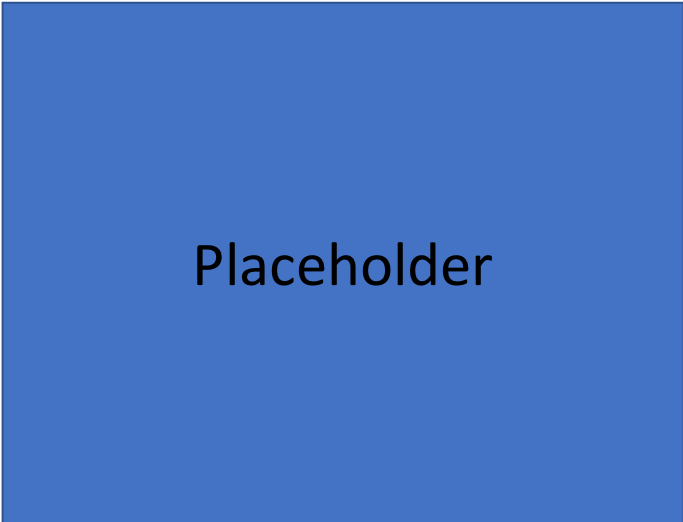
\includegraphics[width=0.7\linewidth]{Chapter3/figure/placeholder.png}
    \caption{Placeholder for classic model fit to comb-drive actuator displacement data at 0.1 mM, 0.5 mM, and 1 mM $KCl$ respectively}\label{classic_circuit_fit}
    \end{center}
\end{figure}

\begin{table}[!htb]
\begin{center}
{\begin{tabular}{|c|c|}
	\hline
	\textbf{Model (i)} & \textbf{Classic Model} \\
     &  \textbf{Assumptions Removed} \\
    \hline
    Leaky Oxide (1) & i) Pure Dielectric Oxide\\
    \hline
    Leaky Oxide  & i) Pure Dielectric Oxide \\
    + Stern (2)    & ii)  No Stern layer \\
    \hline
    Variable Resistor (3) & iii) Constant Bulk Resistor \\
    \hline
    Leaky Oxide+ & i) Pure Dielectric Oxide\\
    Stern+   & ii)  No Stern layer \\
     Variable Resistor (4) & iii) Constant Bulk Resistor  \\
    \hline  
\end{tabular}}
\caption{Hierarchy of models developed in this paper, and the classic circuit model assumptions they address}\label{hiearchy_table}
\end{center}
\end{table}


\section{Novel Circuit Models of Comb-drive Actuator in Electrolytes}
In this section, we outline the development of the set of models summarized in table \ref{hiearchy_table}. In order to represent these models, we re-express the frequency dependence of the force on the comb-drive actuator, \ref{classic_force_comb}, as
\begin{equation}\label{general_red_force_comb}
F = \dfrac{Nb\epsilon_0\epsilon_W}{g}h_i(\omega)V_{AppRMS}^2
\end{equation}
where $h_i$ is the function of frequency that corresponds to the Leaky Oxide, Leaky Oxide + Stern, Variable Resistor, and Leaky Oxide + Stern + Variable Resistor models (i=1,2,3,4). Explicitly, 

\begin{align}\label{gen_freq_eqn}
h_i(\omega) = \bigg|\dfrac{Z_{Bulk}}{Z_{Bulk}+2*Z_i(\omega)}\bigg|^2,  i=1,2,3,4,5
\end{align}

The Leaky Oxide and Leaky Oxide + Stern models yield analytical expressions for $h_i$, while the frequency dependence of the Variable Resistor and Leaky Oxide + Stern + Variable Resistor models are evaluated numerically, after solving systems of ordinary differential equations (ODEs). 
 
The Leaky Oxide and Leaky Oxide + Stern models are created by modifying the interface impedance, $Z_i, i=2,3$. Figures \ref{classic_circuit}, \ref{leaky_ox_circuit}, and \ref{leaky_ox_stern_circuit} shows the circuit model for the Classic, Leaky Oxide, and Leaky Oxide + Stern models. For both the Leaky Oxide, and Leaky Oxide + Stern models, the bulk impedance is a constant value resistor, $Z_{Bulk}=R_{Bulk}$. However, their interface impedances vary. Noting that the leaky oxide and stern layer impedances are 

\begin{equation} \label{oxide_stern_impedances}
Z_{Ox} = \frac{R_{Ox}}{1+j\omega R_{Ox}C_{Ox}}, \quad Z_{Stern} = \frac{1}{j\omega C_{Stern}},
\end{equation}

we can right the interface impedance of the Leaky Oxide + Stern model, and the Leaky Oxide models as 

\begin{align}
Z_{LeakyOx}(\omega) = Z_{Ox}, \label{leaky_ox_imped} \\ 
Z_{LeakyOx+Stern}(\omega) = Z_{Ox}+ Z_{Stern}  \label{leaky_ox_stern_imped}. 
\end{align}

The Variable Resistor and Leaky Oxide + Stern + Variable resistor models are modifications of the Classic and Leaky Oxide + Stern models respectively. Specifically, both of these models remove the assumption that the bulk resistance is constant, and instead model it as a function of bulk concentration. In addition, these models account add the stern layer, and the nonlinear electric double layer to the interface. We note that it is assumed that the concentration in the bulk changes in a manner that is spatially homogeneous. This yields a system of ODEs of the form,

\begin{align} \label{ode_states}
\dot{\mathbf{y}} = f(\mathbf{y},t,\omega), \nonumber\\ \mathbf{y} =[q^*,V_{Ox}^*,V_{St}^*,V_{EDL}^*,V_{Bulk}^*,i^*,c_0^*,R_{Bulk}^*]^T
\end{align}

where  $q$ is the surface charge on the Electric Double Layer (EDL) capacitor, $V_{Ox}^*$  is the voltage drop across the native oxide, $V_{Stern}^*$ is the voltage drop across the stern layer, $V_{EDL}^*$ is the voltage drop across the EDL, $V_{Bulk}^*$ is the voltage drop across the bulk, $i^*$ is the current, $c_0^*$ is the concentration of the bulk electrolyte, and $R_{Bulk}^*$ is the resistance of the bulk. All of these quantities are dimensionless,  and $V_{Bulk}^*$ is re-dimensionalized to $V_{Bulk}$ when evaluating displacement. The ODEs for the Leaky Oxide + Stern + Variable Resistor model are of the same form as equation (7).

The main difference between these models is in the modification of $V_{Ox}^*$ to account for the parallel addition of $R_{Ox}$ to $C_{Ox}$, figures \ref{leaky_ox_circuit}. Unlike for the case of the Leaky Oxide and Leaky Oxide + Stern models, evaluating the functional dependence on force, $h_i(\omega)$, requires numerical integration. Specifically, we use the RMS integral of $V_{Bulk}$ to obtain

\begin{align} \label{numeric_vrms}
V_{RMS}(\omega) = \sqrt[]{\frac{1}{T} \int_{0}^{T}V_{Bulk}(\omega,t)^2dt} = h_i(\omega)V_{AppRMS},\nonumber\\ i = 3,4
\end{align}

\subsection{ODEs for Numeric Circuit Models}
We have introduced abstractly the Variable Resistor, and the Leaky Oxide + Stern + Variable Resistor models. In this section, we enumerate the non-dimensional ODEs that must be solved in order to evaluate these models. For the variable resistor model, the system of ODEs is

\begin{align}
\frac{dq^*}{dt^*} = i^* \label{charge_state} \\
\frac{dV^*_{EDL}}{dt^*} = \frac{i^*}{C_{EDL}^*} \label{vedl_state} \\%\frac{i}{dq/dV_{EDL}} \\
\frac{dV^*_{Stern}}{dt^*} = \frac{i^*}{C_{Stern}^*} \label{vstern_state} \\%\frac{i}{ \frac{C_{Stern} \lambda_{D}}{C_{Water} \lambda_{Stern}}dq/dV_{0}} \\
\frac{dV^*_{Ox}}{dt^*} = \frac{i^*}{C_{Ox}^*} \label{vox_state} \\
\frac{dc^*_0}{dt^*} = -2i^*sign(q^*) \label{concentration_state}\\
\frac{dR^*_{Bulk}}{dt^*} = \frac{-1}{2c_{0}^{*2}}\frac{dc^*_0}{dt^*} \label{resistor_state}\\
\frac{dV^*_{Bulk}}{dt^*} = \frac{di^*}{dt^*}R^*_{Bulk} + i^*\frac{dR^*_{Bulk}}{dt^*}\label{vbulk_state}  \\ 
\frac{di^*}{dt^*} = \frac{\bigg(\frac{dV^*_{Bulk}}{dt^*}-2\frac{d}{dt^*}V^*_{INT}-i^*\frac{dR^*_{Bulk}}{dt^*}\bigg)}{R^*_{Bulk}} \label{current_state} 
\end{align}
where 
\begin{equation}
    V^*_{INT}  = V^*_{EDL}+V^*_{Stern}+V^*_{Ox}   
\end{equation}
 and each state has been defined in the paragraph following \ref{ode_states}. $C_0$ is the dimensionless linear differential capacitance of the electric double layer, \ref{lin_diff_cap}, and $C_{EDL}$ is the dimensionless nonlinear differential capacitance of the electric double layer which is expressed as
\begin{equation} \label{edl_nonlinear}
C_{EDL} = C_{0} cosh\bigg(\frac{V^*_{EDL}}{2}\bigg).
\end{equation}

We note four things. First, the differential equation for the bulk resistor, $R_{Bulk}^*$ is obtained by taking a time derivative of the bulk resistance expressed in \ref{bulk_resist_volt}. Second, with the exception of the $C_{EDL}^*$, the non-dimensional capacitance of circuit element $l$, $C_l^*$, is 

\begin{equation}
    C_l^* = \bigg(\frac{C_{l} \lambda_{D}}{C_{Bulk} \lambda_{l}}C_0\bigg)
\end{equation}
where $C_{l}$ is the dimensional capacitance of the circuit element, $C_{Bulk}=\frac{\epsilon_W}{g}$ is the capacitance of the bulk which is assumed to be calculated based on the relative permitivitty of water, $\lambda_{l}$ is the thickness of the physical layer represented by circuit element $l$, and $\lambda_{D}$ is the debye lenght. Third, the voltages in this system are where non-dimensionalized using the thermal voltage, $V_T$. Finally, the voltage, $V_{l}$, bulk resistor, $R_{Bulk}^*$, capacitances, $C_l^*$, and time $t^*$ are the only parts of the ODE that are explicitly non-dimensionalized. The non-dimensional charge and current fall out of solving the ODEs with these quantities.

The system of ODEs for the Leaky Oxide + Stern + Variable Resistor model is identical to that of the Variable Resistor model, with the exception of a modification to \ref{vox_state} which is rewritten as
\begin{align} \label{vox_state_leakoxstern}
\frac{dV^*_{Ox}}{dt^*} = \frac{i^* - V^*_{Ox}/R^*_{Ox}}{C^*_{Ox}};
\end{align}

\section{Neglected Effects of Novel Models}
Up until this point, we have neglected two key effects in the development of our models. The first is the depletion layer that can develop in doped silicon, and the second is the formation of concentration gradients in the bulk electrolyte. We describe both of these effects in this section, and justify their explicit absence from our models. 

\subsection{Depletion Layer Formation}
The silicon wafers used to fabricate the comb-drive actuators are p-type boron-doped to 0.008-0.01 \textOmega $\textrm{ }cm$. When a voltage is applied to the comb-drive, the resulting external electric field causes charge carriers to collect at the interface of the silicon and native oxide. This region is called the depletion layer, and can also be approximated as a capacitor. The relative importance of this capacitance, compared to other circuit elements in our models, is determined by the width of the depletion layer. We perform a scaling analysis in order to determine the importance of this depletion layer.

Figure \ref{depletion_layer} depicts the depletion layer in series with the native oxide and Stern layers, as well as the bulk electrolyte, for a single comb-drive finger. The analysis detailed in this section assumes that the native oxide is a pure dielectric, and makes use of dimensional quantities. We write Poisson's equation for the depletion layer as
\begin{equation}
\frac{d^2\phi}{dx^2} = -\frac{dE}{dx} = -\frac{e}{\varepsilon_{Si}}(n_+ - n_- + N_d), \quad -x_d \leq x \leq 0
\end{equation}
where $n_+$ and $n_-$ are positive and negative free charge carrier concentrations respectively, and $N_d$ is the concentration of the positive dopant. We solve for the electric field, assuming that there are no free charge carriers in the depletion layer.
\begin{equation} 
E(x) = \frac{eN_d(x+x_d)}{\varepsilon_{Si}}.
\end{equation}
We next require that the electric field be continuous at the interface of the native oxide and the depletion layer, $x=0$. and solve for the depletion layer width, $x_d$.

\begin{figure}[htpb]
    \begin{center}
    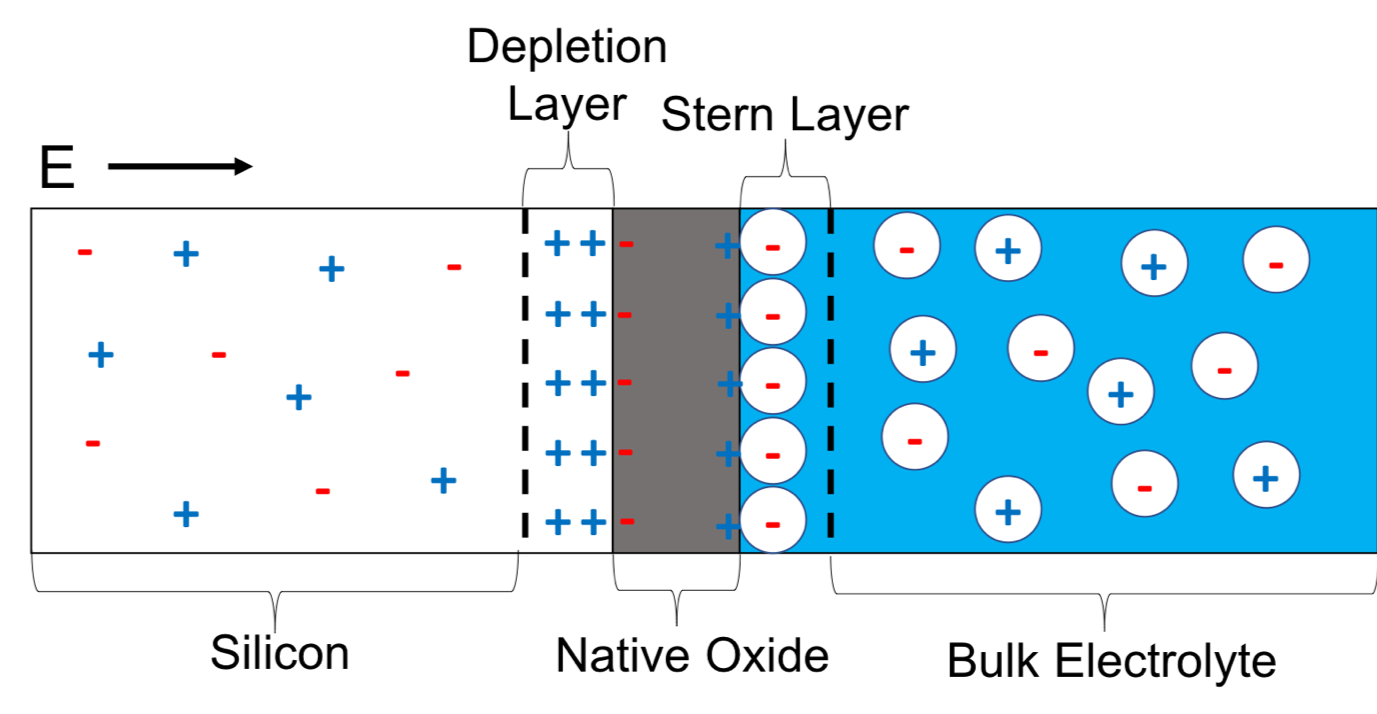
\includegraphics[width=0.7\linewidth]{Chapter3/figure/depletion_layer.png}
    \caption{Illustration of one finger in a pair of comb-drive fingers. It depicts the Silicon substrate, the depletion layer, the native oxide, the Stern Layer, and the bulk electrolyte.}\label{depletion_layer}
    \end{center}
\end{figure}
% \begin{equation}
% E(x=0) = \frac{eN_dx_d}{\varepsilon_{Si}} = \frac{V_{Ox}}{t_{Ox}}.
% \end{equation}
% Re-writing equation (52) allows us to write the depletion layer width as
\begin{equation}
x_d = \frac{\varepsilon_{Si}}{t_{Ox}}\frac{V_{Ox}}{eN_{d}}.
\end{equation}
If we use the nominal values of the physical parameters in equation (51), shown in \ref{table_phys_param_nomvals}, then the depletion layer width is 
\begin{equation}
x_d = 3 \times 10^{-8} V_{Ox}.
\end{equation}
We know that $V_{Ox}$ is at most O(1), so we can approximate the minimum capacitance of the depletion layer as
\begin{equation}
C_{D} \approx \frac{\varepsilon_0 \varepsilon_{Si}}{x_d} = 0.0034 
\end{equation}

\begin{table}[!htb]
\begin{center}
{\begin{tabular}{|c|c|}
	\hline
	\textbf{Physical Parameters} & \textbf{Nominal Values} \\
    \hline
    $\varepsilon_{Si}$ & 11.68 \\
    \hline 
    $t_{Ox}$ & 2 $nm$ \\
    \hline
    $N_d$  & $10^{25} m^{-3}$  \\
    \hline
\end{tabular}}
\caption{Nominal values of physical parameters used for approximated the width of the depletion layer.}\label{table_phys_param_nomvals}
%\begin{flushleft} 
%Table III: 
%\end{flushleft} 
\end{center}
\end{table} 

Since the nominal capacitance of the Stern and native oxide layers are O(0.1) and O(0.01) respectively, it is clear that the effects of the depletion layer capacitance is significant. While this is relevant for conceptualizing the physical system, explicitly modeling the depletion layer does not impact the ability of our reduced models to fit the data. The models presented in this chapter are lumped circuit models, rather than spatial models. As a result, the depletion layer capacitance, which is in series with the Stern or oxide layer capacitance depending on the model, can be lumped in with the capacitance of these layers. When these models are fit, the resulting value of the Stern and oxide capacitance  should be viewed as compensating for both these respective layers and the Depletion layer.

\subsection{Concentration Gradients}
The variable resistor models described in the previous section assumes that the concentration of the electrolytes changes uniformly across the bulk electrolyte, i.e. that the concentration has no gradients. While this is not generally true, the impact of concentration gradients is only relevant when large low-frequency voltages are applied to the bulk. In the case of the comb-drives fabricated for this paper, we postulated that the impedance of the native oxide at low frequencies was sufficiently high enough to prevent this. We confirm in the next chapter that, in the context of our current devices, the variable resistor models that account for concentration gradients fit the data identically to our models that assume uniform concentration. For the sake of completeness, we illustrate here how we account for concentration gradients in our variable resistor model. This derivation is derived based on the work of Bazant et al \cite{Bazant2004}.

Bazant et al. used matched asymptotics to derive expressions for the change in the concentration of a \textit{z:z} electrolyte. They first expressed the dimensionless concentration in the bulk as
\begin{equation} \label{concentration_asympt}
c^* = c_+^* + c_-^* = 2c_0^* + \gamma c_1^*
\end{equation}
where $c_1^*$ accounts for the variation in the bulk concentration, and $\gamma$ is as defined in \ref{lin_diff_cap}. The time derivative of the the bulk concentration is then
\begin{equation} \label{dcdt_asympt}
\frac{dc^*}{dt^*} = \gamma \frac{dc_1^*}{dt^*} = \gamma \frac{d^2c_1^*}{dx^{*2}},
\end{equation}
with the boundary condition
\begin{equation} \label{dcdt_asympt_bc}
\frac{dc_1^*}{dx^*}(x=0,t) = -2 sinh\bigg(\frac{V_{EDL}^*}{2}\bigg) \frac{dV_{EDL}^*}{dt^*}.
\end{equation}
In order to account for the concentration gradient, we replace \ref{concentration_state} with \ref{dcdt_asympt} and \ref{dcdt_asympt_bc}. We finally replace $R_{Bulk}^*$ and $\frac{dR_{Bulk}^*}{dt^*}$ with
\begin{equation}
R_{Bulk}^* = \frac{1}{c^*},
\end{equation}

and 

\begin{equation}
\frac{dR_{Bulk}^*}{dt^*} = \int_{0}^{g^*} \frac{-1}{c^{*2}}\frac{dc^*}{dt^*}dx^*.
\end{equation}
respectively.

\section{Chapter Review and Further Work}
In this chapter, we justified the use of a circuit model to describe the behavior of electrolytes between parallel plates using the PNP equations, detailed the classic circuit model that falls out of this circuit model, as well as the assumptions behind this model, and presented a hierarchy of models that addressed the assumptions of the classic circuit model. Moreover, we noted important effects neglected by our reduced models, and stated that, as will be shown in chapter 4, that these had no impact on describing the comb-drive actuators in electrolytes that were fabricated for this dissertation.

In the future, it would be useful to numerically, and experimentally, explore how changes in the parallel plate system, especially the thickness of the native oxide, would impact the importance of effects neglected by our model.